%********************************************************************
% Appendix
%*******************************************************
% If problems with the headers: get headings in appendix etc. right
%\markboth{\spacedlowsmallcaps{Appendix}}{\spacedlowsmallcaps{Appendix}}
\chapter{Guide for Running SeriChat}{\label{app:test}}
To be able to run SeriChat you just have to run the JAR-file (\texttt{SeriChat.jar}) through the terminal with the below mentioned steps (it is tested on Linux and Mac OSX).
For each step you have to open a new terminal window and navigate to the folder where the \texttt{SeriChat.jar} file is.
\graffito{$\leftarrow$ Important read!}

\section{Step-by-Step Guide}
\begin{enumerate}
	\item \textbf{Create the bootstrapping node} 
				\\\texttt{java -jar SeriChat.jar}
	\item \textbf{Create a group} 
		\\\textit{add groupowners name, -c (for create) , name of group, and password}
		\\\texttt{ java -jar SeriChat.jar Niels -c AU 123456}
		
	\item \textbf{Join a group} 
	\\\textit{add a name for the new member and replace -c with -j (for join)} 
	\\\texttt{java -jar SeriChat.jar Bilal -j AU 123456}
\end{enumerate}

Step 2 and step 3 can be repeated with new names for both the group owners, group members, and new groups.

\section{Example of SeriChat Test Scenario}
On \autoref{fig:demo-screenshot} is shown a screenshot of the demo.
\begin{figure}[bth]
	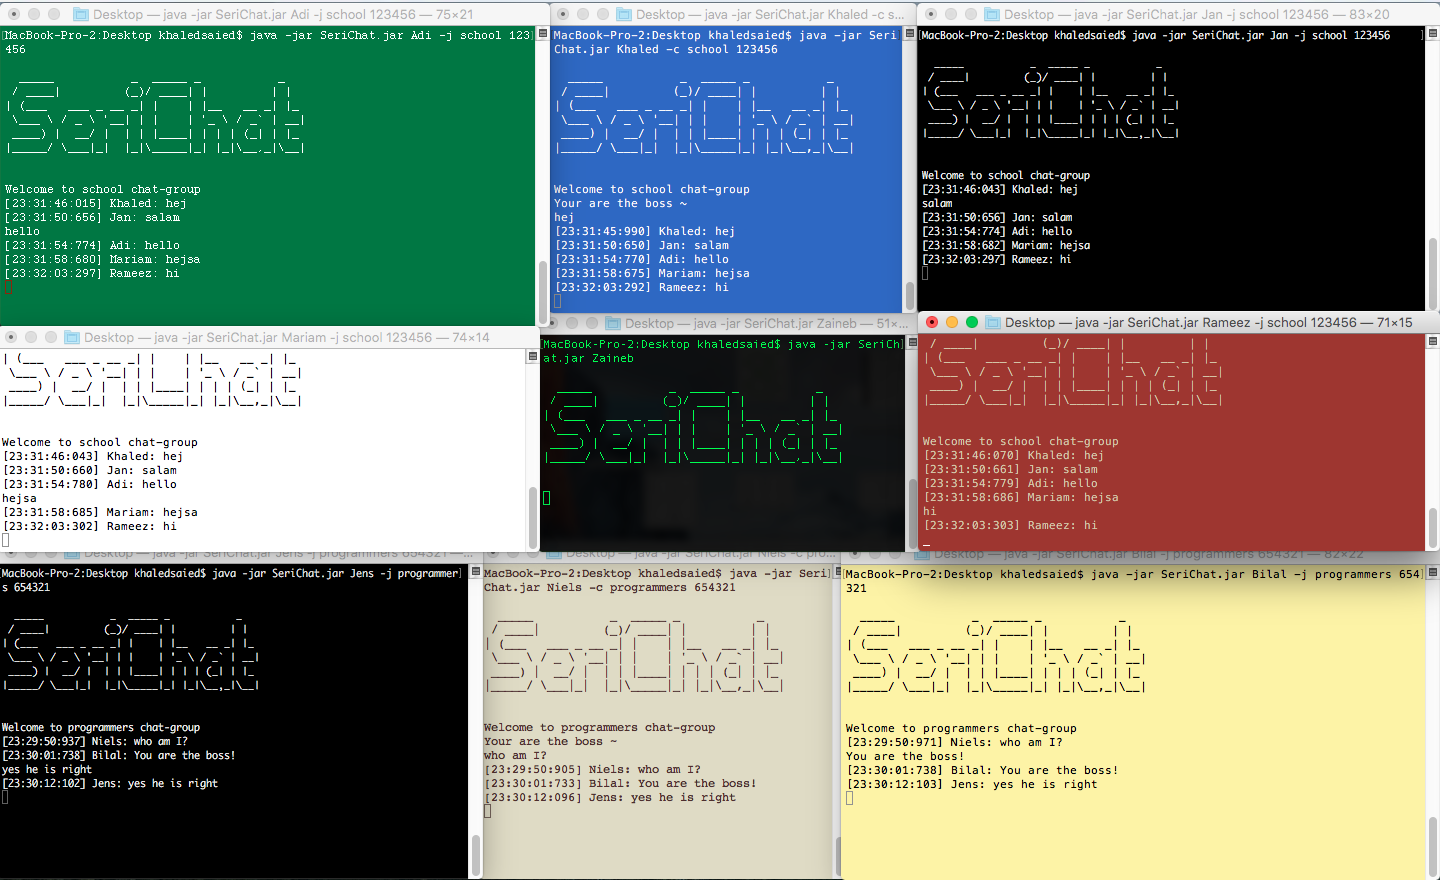
\includegraphics[width=1\linewidth]{gfx/Demo-Screenshot}}
\caption{Screenshot of demo running SeriChat}
{\label{fig:demo-screenshot}
\end{figure}